\documentclass[../ClassicThesis.tex]{subfiles}
\begin{document}

%************************************************
\chapter{Implementation Goals and Toolchain}
\label{ch:toolchain}
%************************************************

\section{The Software Is a Web Service}

Our application {\platener} is a web service. {\platener}
can be used without installation on desktop and mobile
devices. We aim to enable any user to produce 3D~objects
with a laser cutter. We minimize the system requirements of
our software by providing a cross-platform web application.
{\platener} is based on HTML~5, CSS,
{\coffeescript}\footnote{\url{http://coffeescript.org/}} and
WebGL. The web server runs in {\nodejs}. The application is
written in such a way that it can be executed without a
browser in {\nodejs} only. This enables power users to run
{\platener} as a command line interface. Third party
applications can utilize {\platener} by integrating the
{\nodejs} package.

\section{Libraries Improve the Development Experience}

{\javascript} and {\nodejs} are backed by a huge community.
The \name{node package manager} (npm)
ecosystem\footnote{\url{https://www.npmjs.com/}} hosts about
250.000 code packages. By reusing modular code we can
significantly speed up our development process. In the
following, we list the most important tools and libraries
used by {\platener}.

\begin{itemize}
\item {\coffeescript} is an indent-based language which
  transpiles to {\javascript}. It provides useful syntactic
  sugar for function and class definitions.

\item
  \name{React}\footnote{\url{https://facebook.github.io/react/}}
  is a {\javascript} library for building modular
  {\userinterface}s.

\item \name{Redux}\footnote{\url{http://redux.js.org/}} is a
  predictable state container which manages the application
  state in a data-driven way.

\item \name{stylus}\footnote{\url{http://stylus-lang.com/}}
  is a powerful CSS pre-processor. Instead of writing pure
  CSS we can benefit from \name{stylus}' scoping,
  inheritance and mixin features. {\platener} is based on
  the
  \name{Bootstrap~3}\footnote{\url{http://getbootstrap.com/}}
  CSS framework.

\item \name{\threejs}\footnote{\url{http://threejs.org/}}
  provides high-level abstractions of the WebGL API.

\item
  \name{webpack}\footnote{\url{https://webpack.github.io/}}
  is a module bundler. It prepares all source code and
  assets into an deployable package.

\item \name{Grunt}\footnote{\url{http://gruntjs.com/}} is a
  {\javascript} task runner with which we automate our setup
  and build process.
\end{itemize}

\section{Development With a Build System}

{\coffeescript} requires transpilation to {\javascript} and
generation of source maps. \name{stylus} affords
pre-processing to CSS. All dependencies need to be included
into the web site because the browser is not authorized to
access the local filesystem. These processes have to be done
each time a line of code changes or a new package is
installed. We utilize \name{Grunt} and \name{webpack} to
create a build system. A build system is a tool, which
automates the process of compiling a computer program
\cite{build-system}. Figure~\ref{} gives an overview of our
toolchain.
\note{include this image here correctly}
% \begin{figure}[h]
%   \centering
%   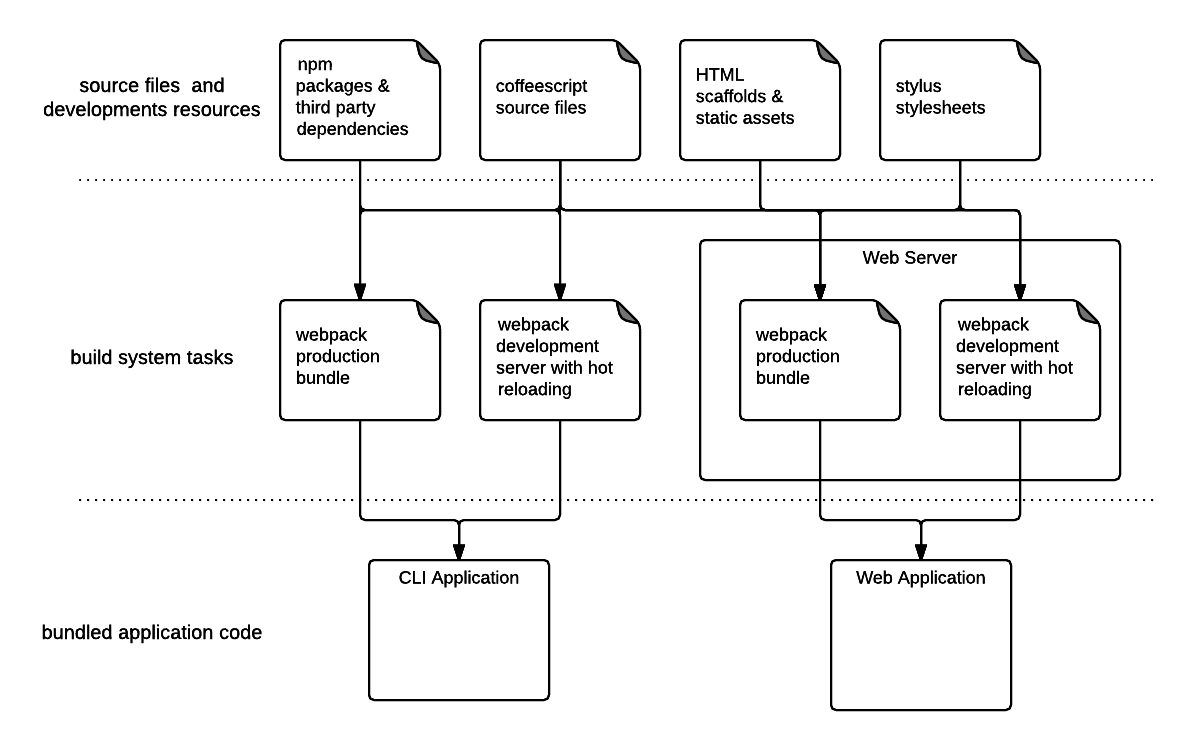
\includegraphics[width=\textwidth]{025-toolchain.jpg}
%   \caption{Toolchain and build system of {\platener}.}
%   \label{fig:toolchain}
% \end{figure}

With our setup the code automatically rebuilds when files
are changed by a developer. Once the new code is built, the
sources are loaded into the browser. Loading sources from
the server can take several seconds. We reduce the waiting
time by performing hot reloads. A hot reload patches the
existing and already loaded code base with a change set.
This greatly improves the development speed.


% {\coffeescript} transpiles to {\javascript}. In order to
% write web applications we are required to use a
% {\javascript} based programming language because browsers
% run on {\javascript} virtual machines. Some parts of our
% application are based on previous work written in
% {\coffeescript} by \citeauthor{bachelor-thesis}. We
% benefited from their legacy system and continued with
% {\coffeescript}. Similar to {\es6}, {\coffeescript} provides
% useful syntactic sugar for function and class definitions.
% \citeauthor{bachelor-thesis} choosed {\coffeescript} because
% {\es6} was not supported by all major browser
% \cite{compat-js}.




% \subsection{Cross-Platform Browser Application}

% \begin{itemize}
% \item web service
% \item cross platform
% \item no installation necessary
% \item target group: makers, run in labspaces, everywhere
% \item typical HTML, CSS, Javascript trio
% \end{itemize}

% \subsection{Headless Version for Integration with Other Software}

% \begin{itemize}
% \item same service without visuals
% \item batch processing or single
% \item idea: integrate with other 3d editing applications to benefit
%   from platener conversions
% \item running on nodejs v 012
% \end{itemize}

% \section{Technologies and Libraries}


% We use the Web Graphics Library (WebGL), because we want our
% rendering results to have sophisticated visual effects. With
% the use of WebGL we can process data on the GPU and execute
% special effects code (shader code) in
% web-browsers~\cite{mdn-webgl}.

% On top of WebGL we use
% {\threejs}\footnote{\url{http://threejs.org}}. {\threejs} is
% a {\javascript} library, which wraps the WebGL API to make
% the usage of WebGL simpler. It provides a scene graph
% implementation. {\threejs} data representations are used
% throughout {\convertify}.


% \begin{itemize}
% \item web service -> necessarily javascript
% \item coffeescript preprocessing, no es6 because previous code base
%   brickify was written in coffeescript -> save effort of rewrites
% \item webgl -> rendering, now almost all major browser support it

% \item nodejs for headless version/ server (backend) support (v0.12
%   because old brickify dependencies)
% \item threejs -> most acknowledged 3d web library (scene graphs and
%   webgl)
% \item bluebird -> promises (nice tech in js to handle async behavior,
%   better than natives because of error handling, more features)
% \item polyfills -> more cross platform support and isomorphic =>
%   browsers and nodejs run in different vms
% \item styles with stylus lib (also taken from brickify)
% \end{itemize}

% \section{Build System and Development Setup}

% \begin{itemize}
% \item gruntfile -> and webpack
% \item different setups for client, server and cli in prod/ dev mode
% \item test runner using mocha
% \item bundle code into minified code and output sourcemaps (nice for
%   in browser debugging)
% \item smart server (rebuilding on filechanges, hotreloading (not
%   compiling everything again for speedup))
% \item browser lifereload (code change immediatly displayed in browser)
% \item react hotreloading -> display changes in ui even without a
%   browser reload (super fast feedback loop)
% \end{itemize}

\end{document}

%%% Local Variables:
%%% mode: latex
%%% TeX-master: "../ClassicThesis"
%%% TeX-command-extra-options: "-shell-escape"
%%% End:
